\documentclass{report}
\usepackage{setspace}
%\usepackage{subfigure}

\pagestyle{plain}
\usepackage{amssymb,graphicx,color}
\usepackage{amsfonts}
\usepackage{latexsym}
\usepackage{a4wide}
\usepackage{amsmath}

\newtheorem{theorem}{THEOREM}
\newtheorem{lemma}[theorem]{LEMMA}
\newtheorem{corollary}[theorem]{COROLLARY}
\newtheorem{proposition}[theorem]{PROPOSITION}
\newtheorem{remark}[theorem]{REMARK}
\newtheorem{definition}[theorem]{DEFINITION}
\newtheorem{fact}[theorem]{FACT}

\newtheorem{problem}[theorem]{PROBLEM}
\newtheorem{exercise}[theorem]{EXERCISE}
\def \set#1{\{#1\} }

\newenvironment{proof}{
PROOF:
\begin{quotation}}{
$\Box$ \end{quotation}}



\newcommand{\nats}{\mbox{\( \mathbb N \)}}
\newcommand{\rat}{\mbox{\(\mathbb Q\)}}
\newcommand{\rats}{\mbox{\(\mathbb Q\)}}
\newcommand{\reals}{\mbox{\(\mathbb R\)}}
\newcommand{\ints}{\mbox{\(\mathbb Z\)}}

%%%%%%%%%%%%%%%%%%%%%%%%%%


\title{{\vspace{-14em} 
\includegraphics[scale=0.4]{ucl_logo.png}}\\
{{\Huge Machine Learning on Options Pricing}}\\
{\large Optional Subtitle}\\
}
\date{Submission date: 1 April 2020}
\author{Wenwen Zheng\thanks{
{\bf Disclaimer:}
This report is submitted as part requirement for the BSc Computer Science at UCL. It is
substantially the result of my own work except where explicitly indicated in the text.
\emph{Either:} The report may be freely copied and distributed provided the source is explicitly acknowledged
\newline  % \\ messes it up
\emph{Or:}\newline
The report will be distributed to the internal and external examiners, but thereafter may not be copied or distributed except with permission from the author.}
\\ \\
BSc Computer Science\\ \\
Dr Dariush Hosseini }



\begin{document}
 
\onehalfspacing
\maketitle
\begin{abstract}
This report will provide an overview on fast substitutions to traditional option pricing techniques using DL. In particular, to examine current approaches. Starting with the ‘Deep Learning for Option Pricing’[Robert Culkin & Sanjiv R. Das] and ‘Supervised Deep Neural Networks’[Tugce Karatas, Amir Oskoui, Ali Hirsa], comparisons and assessments can be made in order to generate new ideas from their inspirations and verify my own findings. 

\end{abstract}
\tableofcontents
\setcounter{page}{1}


\chapter{Introduction}
This chapter includes information which covers the big picture of the project, it should include:
\begin{itemize}
\item Motivation; Why this area etc
\item My hypothesis tests
\item Summaries of how I will approach the problem
\item The scope and products of interests
\end{itemize}

\section{Aims and Possible Applications}
Chapters should contain numbered sections and sub-sections.

\section{Project Overview}
Chapters should contain numbered sections and sub-sections.

\section{Section 1}
Chapters should contain numbered sections and sub-sections.

\section{Mathematical Notation}
Mathematical expressions are placed inline between dollar signs, e.g. $\sqrt 2, \sum_{i=0}^nf(i)$, or in display mode
\[ e^{i\pi}=-1\] and another way, this time with labels,
\begin{align}
\label{line1} A=B\wedge B=C&\rightarrow A=C\\
&\rightarrow C=A\\
\intertext{note that}
n!&=\prod_{1\leq i\leq n}i \\
\int_{x=1}^y \frac 1 x \mathrm{d}x&=\log y
\end{align}
We can refer to labels like this \eqref{line1}.   

\chapter{Literature Review}

This Chapter contains my research and reading on both options pricing and DL and current DL on options pricing.

\section{Options and Options Pricing}
Often lots of citations here (and elsewhere), e.g. \cite{Rey:D} or \cite[Theorem 2.3]{PriorNOP70}.   Bibtex can help with this, but is not essential. If you want pictures, try

\begin{center}
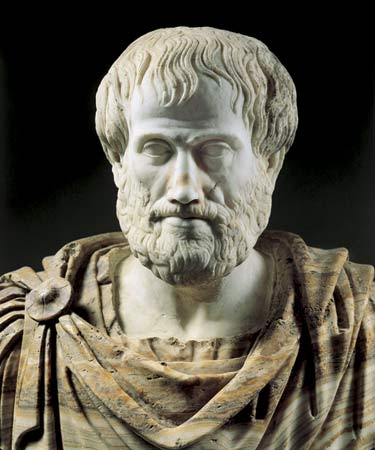
\includegraphics[scale=.5]{aristotle.jpg}
\end{center}
You can use 
\begin{itemize}
\item lists
\item like this
\end{itemize}
or numbered
\begin{enumerate}
\item like this,
\item or this
\end{enumerate}
but don't overdo it.

\section{Deep Learning}
\subsection{Deep Learning in general}
Explain Deep Learning in a simple way\\
Types of Deep Learning (Methods to be used in this report)
\subsection{Deep Learning in Finance & Options Pricing}


\chapter{Data and Pre-processing}
This Chapter contains everything with synthetic data for all experiments;
vanilla options;\\
Monte-Carlo;\\
Exotic options'\\

\begin{definition}\label{def}
See definition~\ref{def}.
\end{definition}
\begin{theorem}
For all $n\in\nats,\; 1^n=1$.
\end{theorem}
\begin{proof}
By induction over $n$.
\end{proof}

\chapter{Experiments with Different Methods}

\section{Deep Learning Model for Option Pricing}
Focus on Deep Learning for Option Pricing’[Robert Culkin & Sanjiv R. Das]\\
Re-implement the DL model on vanilla options and produce the suggested test results\\
Implement traditional Monte-Carlo methods for the same vanilla options \\
Assessments on performances - speed (various data size), accuracy, Greek stability etc
Based on results, make improvements and suggest different user cases\\
Train the DL model and the traditional method for exotic options\\
Run tests and comparisons again for new conclusions

\subsection{DL Implementation on Vanilla options}
\subsection{Implementation of  traditional Monte-Carlo method}
\subsection{Examination with Traditional Methods}
\subsection{Extension to Exotic Options Pricing}

\section{Supervised Deep Neural Network (DNN)}
Focus on ‘Supervised Deep Neural Networks’[Tugce Karatas, Amir Oskoui, Ali Hirsa]\\
Train the supervised DNN model suggested in the paper and make variations to work for both vanilla options and exotic options\\
Run assessments during several stages and draw conclusions along the process

\subsection{DNN Implementation on Vanilla options}
\subsection{Examination with Traditional Methods}
\subsection{Extension to Exotic Options Pricing}

\section{Possible extensions on CVA}
\subsection{Implementation Details}
\subsection{Result Analysis}


\chapter{Conclusions}
\section{Achievements and Deliverables}
Summarise the achievements to confirm the project goals have been met.
\section{Evaluation}
Evaluation of the work (this may be in a separate chapter if there is substantial evaluation).
\section{Future Work}
How the project might be continued, but don't give the impression you ran out of time!

\appendix


\begin{thebibliography}{HHM99}


\bibitem[Pri70]{PriorNOP70}  %only an example
A.~Prior.
\newblock The notion of the present.
\newblock {\em Studium Generale}, 23:  245--248, 1970.


\bibitem[Rey97]{Rey:D}
M.~Reynolds.
\newblock A decidable temporal logic of parallelism.
\newblock {\em Notre Dame Journal of Formal Logic}, 38(3):  419--436,
  1997.
\end{thebibliography}
\chapter{Other appendices, e.g., code listing}
Put your appendix sections here

\end{document}